\chapter{EMC, SRC and Scaling Violations}

    From Rey’s thesis:
    scale separation at short distances - nucleons that are paired (SRC) only care  about eachother - factorize wavefunction into 2-body wavefunctin and A-2 nucleus wavefunction. Analogy of 2 dancers dancing together, don;t care about anyone else in the room

    \section{EMC and SRC}
        \subsection{EMC}
            EMC effect - named after European Muon Collaboration, is the observed effect that when taking the ratio of the $F_2$ structure functions of iron vs. deuterium and observe behavior over x, that there is a drop in the ratio from x = 0.3 to x = 0.7.
            \begin{figure}[H]
                \centering
                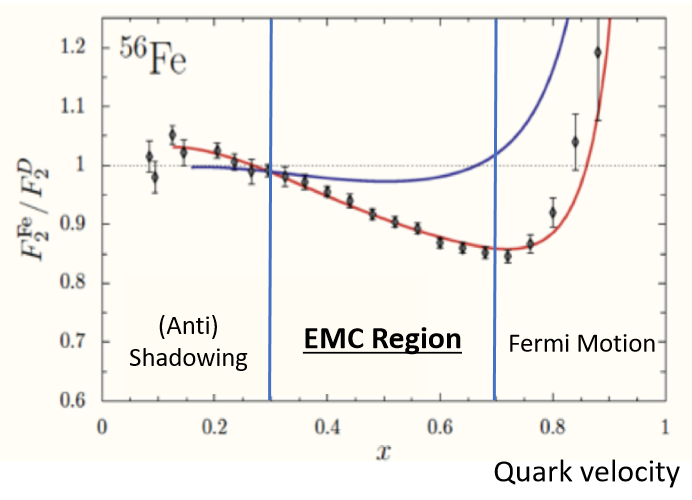
\includegraphics[width=11cm]{NuclearPhysics/pics/EMC_SRC_Scaling/EMC_Fe.PNG}
            \caption{NN Interaction Potential}
            \end{figure}
            
    \section{scaling violations in DIS}




    \section{Proton Radius Puzzle}
        Two methods to measure the proton radius are elastic electron-proton scattering and the spectroscopy of hydrogen atoms. It can be measured by Rosenbluth separation in ep scattering. In 2010 new method using muonic hydrogen found a substantial discrepancy compared to the previous results. Muonic hydrogen is more precise because the Lamb shift is several million times more sensitive to the proton radius sense teh muon is about 200 times closer to the proton than in normal hydrogen. A fundamental difference between e-p and mu-p interactions could explain the discrepancy, but this is unlikely based on other experimental constraints.\\
        \newline
        \indent PRad aimed to resolve this - high-precision e-p scattering. Magnetic spectrometer free method with windowless hydrogen gas target. It uses a calorimeter based method instead of a spectrometer. It measures down to Q2 values of $wx10^{-4}$, which is crucial to get to low values as the radius is determined as the slope of the form factor at Q2 = 0. \\
        
            \begin{figure}[H]
                \centering
                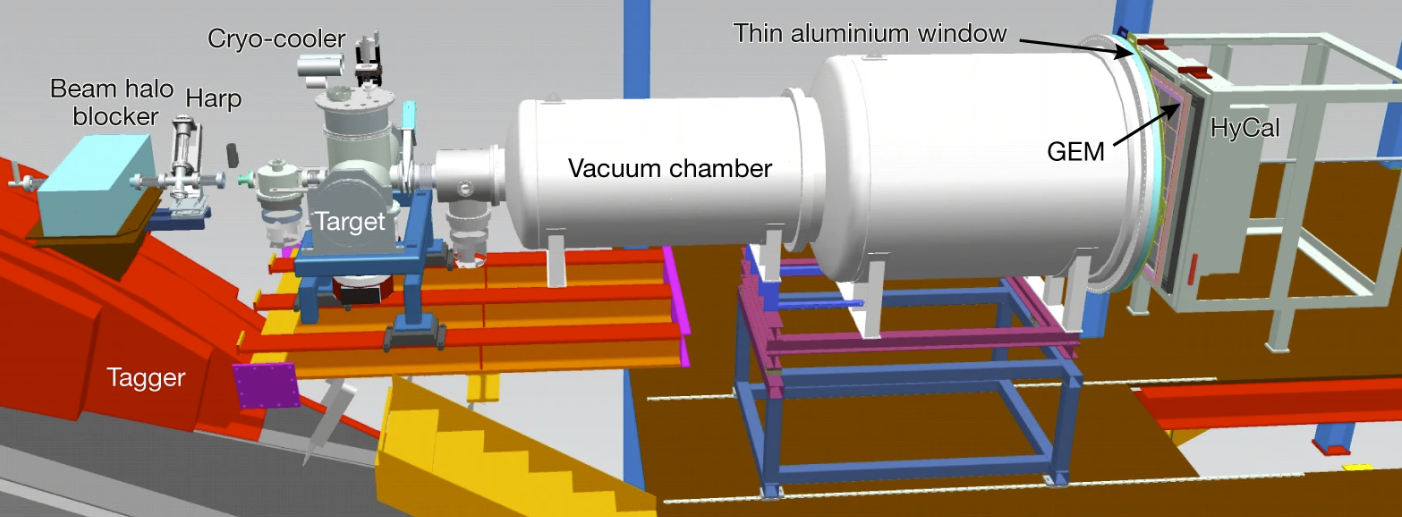
\includegraphics[width=11cm]{NuclearPhysics/modules/emc-src-scaling/pics/prad-setup.PNG}
            \caption{PRad Experimental Setup}
            \end{figure}
        
        The experimental setup was a 4cm long windowless liquid gas target, a hybrid electromagnetic calorimeter, a GEM plane in front of the calorimeter, and 5 meters of space between target and detectors. Beam energy 1.1 and 2.2 GeV. Took place in Hall B. \\
        Why is this detector set up better than a spectrometer? Unclear!
        
            \begin{figure}[H]
                \centering
                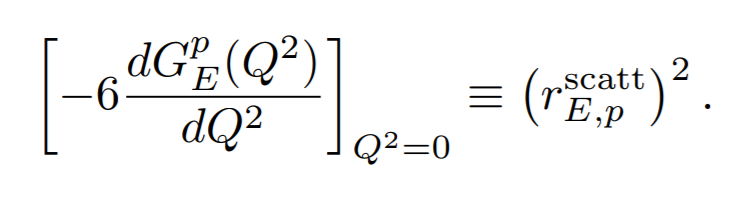
\includegraphics[width=11cm]{NuclearPhysics/modules/emc-src-scaling/pics/prad-GE.PNG}
            \caption{PRad Functional Principle}
            \end{figure}
        
        Nevermind the slope of Prad, the actual form factor GE that PRad measured was different than what others measured, which hints to some other difference? Richard btw thinks this actually may not be an issue, e.g. the proton radius is only well defined in its own rest frame, and hard scattering in ep collisions is not a proton rest frame, among other issues in comparing the two measurements: \href{https://arxiv.org/pdf/1806.10475.pdf}{paper}.
        
        Yimin's experiment at Mainz is set up to measure GE at very low Q2, which isn't measuring the proton radius, but is just trying to compare to PRad at one level up. 
        
        \href{https://www-nature-com.libproxy.mit.edu/articles/s41586-019-1721-2?fbclid=IwAR3edCOsl_PqnQiqe2SQDxfcDS2MutChCfLUiEzHh6y5cjIdKXjuhqiC8d0}{Nature PRad Paper}
